\section{Introduction}
The observed range of bacterial growth rates is enormously diverse. In
natural environments, some microbial organisms might double only once per
year \citep{mikucki2009} while in comfortable laboratory conditions, growth
can be rapid with several divisions per hour \citep{schaechter1958}. This six
order-of-magnitude difference in time scales encompasses different microbial
species and lifestyles, yet even for a single species such as \textit{Escherichia
coli}, the growth rate can be modulated over a similar scale by tuning the
type and amount of nutrients in the growth medium. This remarkable
flexibility in growth rate illustrates the intimate relationship between
environmental conditions and the rates at which cells convert nutrients into
new cellular material -- a relationship that has remained a major topic of
inquiry in bacterial physiology for over a century \citep{jun2018}.

As was noted by Jacques Monod, ``the study of the growth of bacterial
cultures does not constitute a specialized subject or branch of research, it
is the basic method of Microbiology.’’ Those words ring as true today as they
did when they were written 70 years ago \citep{monod1949}. Indeed, the study
of bacterial growth has undergone a renaissance. Many of the key questions
addressed by the pioneering efforts in the middle of the last century can be
revisited by examining them through the lens of the increasingly refined
molecular census that is available for bacteria such as the microbial
workhorse \textit{E. coli}. In this work, we explore an amalgamation
of recent proteomic data sets to explore fundamental limits of bacterial growth.

Several of the evergreen questions about bacterial growth that were originally
raised by microbiologists in the middle of the 20th century can now be reframed
in light of this newly available data. For example, what biological
processes set the absolute speed limit for how fast bacterial cells can grow and
reproduce? How do cells alter the absolute numbers and relative ratios of their
molecular constituents as a function of changes in growth rate or nutrient
availability? In this paper, we address these two questions from two distinct
angles. First, as a result of an array of high-quality proteome-wide
measurements of the \textit{E. coli} proteome under myriad growth
conditions, we have a census that allows us to explore how the number of key
molecular players change as a function of growth rate. Here, we have compiled
a combination of \textit{E. coli} proteomic data sets collected over the past decade using
either mass spectrometry \citep{schmidt2016, peebo2015, valgepea2013} or
ribosomal profiling \citep{li2014} across 31 unique growth conditions (see Appendix \nameref{sec:SI_exp_summary} for further discussion
of these data sets). Second, by
compiling molecular turnover rate measurements for many of the fundamental
processes associated with bacterial growth, we make quantitative estimates
of key cellular processes (schematized in \FIG{categories}) to determine whether the observed protein copy numbers under varying conditions
appear to be in excess of what would be minimally required to support cell
growth at the observed rates.
The census, combined with these estimates, provide a
window into the question of whether the rates of central processes such as
energy generation or DNA synthesis are regulated systematically as a function of
cell growth rate by altering protein copy number in individual cells.

% Throughout this paper we make a series of order-of-magnitude estimates for the copy
% numbers and growth rate dependent expression of a variety of key
% processes required for growth, schematized in \FIG{categories}.
% , informed by the collection of
% proteomic data sets.
% We use these estimates to explore which, if any, of the
% hypothesis illustrated in \FIG{categories} act as molecular bottlenecks
% that limit bacterial growth.
% Specifically, we leverage a combination of
% \textit{E. coli} proteomic data sets collected over the past decade using
% either mass spectrometry \citep{schmidt2016, peebo2015, valgepea2013} or
% ribosomal profiling \citep{li2014} across 31 unique growth conditions.

Throughout our estimates, we consider a modest growth rate of $\approx$ 0.5
hr$^{-1}$ corresponding to a doubling time of $\approx$ 5000 seconds, as the the
data sets heavily sample this regime. While we formulate point estimates for the
complex abundances at this division time, we consider how these values will vary
at other growth rates due to changes in cell size, surface area, and chromosome
copy number \citep{taheriaraghi2015}. Broadly, we find that for the majority of
these estimates, the protein copy numbers appear well-tuned for the task of cell
doubling at a given growth rate. It emerges that translation, particularly
of ribosomal proteins, is the most plausible candidate for a molecular
bottleneck. We reach this conclusion by considering that translation is 1) a
rate limiting step for the \textit{fastest} bacterial division, and 2) a major
determinant of bacterial growth across the nutrient conditions we have
considered under steady state, exponential growth. This  enables us to suggest
that the long-observed correlation between growth rate and cell size
\citep{schaechter1958, si2017} can be simply attributed to the increased
absolute number of ribosomes per cell under conditions supporting extremely
rapid growth, a hypothesis which we formally mathematize and explore.

% First, we consider potential limits on the transport
% of nutrients into the cell. We address this hypothesis by performing an
% order-of-magnitude estimate for how many carbon, phosphorus, and sulfur atoms
% are needed to facilitate this requirement. As a second hypothesis, we consider
% the possibility that there exists a fundamental limit on how quickly the cell
% can generate ATP. We approach this hypothesis from two angles, considering how
% many ATP synthase complexes must be needed to churn out enough ATP to power
% protein translation, followed by an estimation of how many electron transport
% complexes must be present to maintain the proton motive force. A third class of
% estimates considers the need to maintain the size and shape of the cell through
% the construction of new lipids for the cell membranes as well as the glycan
% polymers which make up the rigid peptidoglycan. Our final class of hypotheses
% centers on the synthesis of a variety of biomolecules. Our focus is primarily on
% the stages of the central dogma as we estimate the number of protein complexes
% needed for DNA replication, transcription, and protein translation.


% This perspective is
% consistent with the linear correlation observed between growth rate and
% ribosomal content (typically quantified through the ratio of RNA to protein) for
% fast growing cells \citep{bremer2008, scott2010}, but also suggest a more prominent role for
% ribosomes in governing the changes in cell size and doubling time across all
% conditions of nutrient limitation.

% Here we
% again leverage the quantitative nature of this data set and present a
% quantitative model of the relationship between the fraction of the proteome
% devoted to ribosomes and the speed limit of translation, revealing a fundamental
% tradeoff between the translation capacity of the ribosome pool and the maximal
% growth rate.

% with single-cell and single-protein resolution using modern methods of video
% microscopy \citep{si2017,harris2018} and through advances in mass spectrometry and
% sequencing technologies \citep{schmidt2016,li2014}. This has permitted
% quantitative insight into how bacteria like \textit{E. coli} allocate their
% cellular resources under nutrient-limitation, and following genomic and
% pharmacological perturbations \citep{scott2010,hui2015,basan2015}.
% This body of experimental data places us in the auspicious position to
% explore how the abundance of essential protein complexes are related to the
% growth rate of the population and interrogate what biological processes may set
% the speed limit of bacterial growth.

% In this work, we seek to leverage a collection of proteomic data sets of
% \textit{Escherichia coli} across 31 growth conditions \citep{valgepea2013,li2014,
% peebo2015,hui2015,schmidt2016} to quantitatively explore what biological
% processes may set the speed limit of bacterial growth.


\begin{figure}
    \centering{
    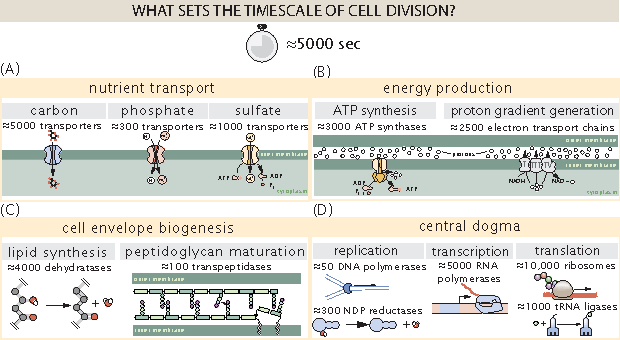
\includegraphics{main_figs/schematic_categories_grouped.pdf}
    \caption{\textbf{Transport and synthesis processes necessary for cell division.}
            We consider an array of processes necessary for a cell to double its
            molecular components, broadly grouped into four classes. These
            categories are (A) nutrient transport across the cell membrane, (B)
            energy production (namely, ATP synthesis), (C) cell envelope
            biogenesis, and (D)  processes associated with the central dogma.
            Numbers shown are the approximate number of complexes of each type
            observed at a growth rate of 0.5 hr$^{-1}$, or a cell doubling time
            of $\approx$ 5000 s.}
    \label{fig:categories}
    }
\end{figure}
